\documentclass{article}

\usepackage{amsmath,amssymb}
\usepackage{fontspec}
\usepackage{unicode-math}

\usepackage{placeins}
\usepackage{graphicx}
\usepackage[font=small,labelfont=bf,textfont=it]{caption}


\usepackage{hyperref}
\hypersetup{hidelinks}

\setcounter{secnumdepth}{2}
\setlength{\emergencystretch}{3em}
\usepackage[a4paper,margin=2.5cm]{geometry}

\graphicspath{{../reports/}}


\begin{document}

\begin{titlepage}
\thispagestyle{empty}
\centering

\vspace*{0.2cm}

\includegraphics[width=0.75\textwidth]{logo_unimi.jpg}
\vspace{2.2cm}


{\LARGE\bfseries
Convolutional Neural Network Architectures for\\[0.3em]
Rock--Paper--Scissors Image Classification\par}

\vspace{0.7cm}
{\normalsize End-Of-Course Project\par}

\vspace{2.0cm}

{\normalsize Leila Cielok\par}

\vspace{0.5 cm}
{\normalsize Data Science for Economics (Master's Degree)\par}
{\normalsize II Year\par}

\vfill

    \begin{quote}
    \small\itshape
    I declare that this material, which I now submit for assessment, is entirely my
    own work and has not been taken from the work of others, save and to the extent
    that such work has been cited and acknowledged within the text of my work. I
    understand that plagiarism, collusion, and copying are grave and serious offences
    in the university and accept the penalties that would be imposed should I engage
    in plagiarism, collusion or copying. This assignment, or any part of it, has not
    been previously submitted by me or any other person for assessment on this or any
    other course of study.
    \end{quote}

    \vfill
    {\large February 28, 2026\par}

\end{titlepage}


\begin{abstract}
This project investigates the impact of architectural complexity on the performance and 
robustness of convolutional neural networks for image classification, using the 
Rock--Paper--Scissors hand gesture task as a controlled case study. Three CNN architectures 
with progressively increasing capacity are designed and compared under identical training 
conditions, including consistent data preprocessing, augmentation, and optimization strategies. 
Model selection is guided by a constrained hyperparameter tuning procedure based on validation 
accuracy. Beyond standard in-distribution evaluation, particular emphasis is placed on 
generalization under domain shift through testing on an external dataset of unconstrained, 
real-world images. The experimental results reveal a clear relationship between model capacity 
and in-distribution performance, while also highlighting that strong validation accuracy does 
not necessarily guarantee robustness to distributional changes. The findings underscore the importance 
of evaluating neural network models beyond held-out validation data when assessing their 
reliability in real-world deployment scenarios.
\end{abstract}


\newpage
\section{Introduction}

Convolutional Neural Networks (CNNs) have become a standard approach for image
classification tasks due to their ability to automatically learn hierarchical
feature representations from raw visual data. In recent years, CNN-based models
have demonstrated strong performance across a wide range of computer vision
applications, from object recognition to gesture and action classification.

Despite these successes, the relationship between architectural complexity and
model generalization remains a central issue in deep learning. While increasing
model capacity often leads to improved performance on held-out validation data,
it does not necessarily translate into robust behaviour when models are exposed
to distributional shifts or unconstrained real-world inputs. This challenge is
particularly relevant for vision tasks involving variability in lighting,
backgrounds, and acquisition conditions, such as hand gesture recognition.

Within this context, the present study uses the Rock--Paper--Scissors image
classification task as a controlled benchmark to analyse how different CNN
architectures behave as model complexity increases. By comparing multiple
architectures under a consistent experimental protocol, the project aims to
provide insight into how architectural choices affect learning dynamics,
error structure, and generalization properties under both standard and shifted
data distributions.

The remainder of the report is organized as follows. Section~2 describes the
dataset and preprocessing pipeline, Section~3 presents the model architectures
and experimental results, and Section~4 discusses generalization under domain
shift.

\section{Data Exploration and Preprocessing}
\subsection{Dataset Description and Exploratory Analysis}

The dataset used in this project was obtained from a publicly available
Kaggle repository (\url{https://www.kaggle.com/datasets/drgfreeman/rockpaperscissors}) 
containing images of hand gestures for the
Rock--Paper--Scissors game. The dataset consists of a total of 2,188 RGB images,
evenly distributed across the three target classes: rock (726 images),
paper (710 images), and scissors (752 images). All images were captured
against a green background under relatively consistent lighting and
white balance conditions, resulting in a visually homogeneous and
well-curated dataset.

Each image is stored in PNG format with an original resolution of 300 ×
200 pixels and is organized into class-specific subdirectories, enabling
a straightforward mapping between file structure and class labels. An
initial exploratory analysis confirmed the near-balanced class
distribution and the absence of missing or corrupted files. Random
visual inspection of samples from each class further revealed that the
hand gestures are generally well-centered and clearly distinguishable,
with limited intra-class variability compared to real-world acquisition
scenarios. This level of consistency makes the dataset particularly
suitable for controlled experiments focused on architectural comparisons
rather than robustness to extreme visual noise.

To avoid any form of data leakage, external datasets are introduced only at a
later stage of the analysis. These datasets are used exclusively for evaluation
and play no role in model training or model selection, allowing generalization
to be assessed independently of the training distribution.

\subsection{Train -- Validation Split}

The dataset was split into training and validation subsets using a
stratified sampling strategy, with 80\% of the images allocated to
training and 20\% reserved for validation. Stratification was performed
at the file level to preserve the original class proportions in both
splits and to guarantee that all classes are represented in each subset.

A fixed random seed was used to ensure reproducibility of the split
across runs. The validation set was held out entirely from training and
used exclusively for model selection, hyperparameter tuning, and
performance evaluation. This splitting strategy provides a reliable
estimate of in-distribution generalization while maintaining
methodological transparency and repeatability.

\subsection{Image Preprocessing: Resizing and Normalization}

After splitting the dataset into training and validation subsets, a
common preprocessing pipeline was applied to all images: to ensure compatibility with convolutional neural network architectures
and to standardize the input space, images were resized to a fixed
square resolution of 96 × 96 pixels. Resizing was performed using
bilinear interpolation with antialiasing, preserving the essential
spatial structure of the hand gestures while reducing computational cost
and memory requirements.

Following resizing, pixel intensities were converted to floating-point
format and normalized to the {[}0, 1{]} range, with the aim of facilitating
stable and efficient optimization by preventing large gradient magnitudes 
during training. This normalization step was applied directly within 
the data pipeline rather than as a dedicated rescaling layer inside the 
models, ensuring consistent preprocessing across all architectures and 
simplifying model definitions.

\subsection{Data Augmentation}

Although the dataset is visually consistent and relatively clean, light
data augmentation was applied during training to encourage better
generalization and to reduce sensitivity to small spatial variations.
Augmentation operations were deliberately kept mild to avoid introducing
unrealistic distortions, given the already constrained nature of the
dataset.

Specifically, the training pipeline includes random horizontal flips,
small rotations, zooming, translations, and slight contrast adjustments, 
applied exclusively to the training set to ensure that validation data remains untouched and
representative of the original distribution. These transformations are applied
on-the-fly at batch loading time, meaning that each epoch exposes the model 
to a different randomized version of the same training samples. This strategy allows the
models to learn more robust feature representations while preserving a
fair and unbiased evaluation protocol.

\section{CNN Architecture and Training}
\subsection{Design of CNN Architectures with Incremental Complexity}

The three convolutional neural network architectures evaluated in this 
study were explicitly designed to form a controlled complexity hierarchy, 
in which representational capacity, depth, and regularization mechanisms 
are progressively increased while keeping the input resolution and 
training protocol fixed.

Model A is a deliberately lightweight architecture intended as a minimal 
baseline. It relies on a small number of depthwise-separable convolutional 
layers followed by max-pooling and a shallow fully connected head. The use 
of separable convolutions significantly reduces the number of trainable 
parameters and computational cost, enforcing a strong inductive bias toward 
learning coarse, low-level spatial patterns. A global average pooling layer 
is employed before the dense classifier, further limiting the model's 
capacity to memorize spatially localized features. As a result, model A 
primarily captures global shape cues rather than fine-grained gesture details.

Model B represents a modest increase in expressiveness and corresponds to 
a conventional shallow CNN. It employs standard convolutional layers 
followed by max-pooling and a fully connected classifier operating on 
flattened feature maps. Compared to model A, this design substantially increases 
parameter count and spatial flexibility, but lacks explicit architectural 
regularization mechanisms beyond implicit constraints imposed by depth 
and pooling. This makes model B more expressive but also more prone to 
sensitivity under distributional shifts, as later evidenced in the 
out-of-distribution evaluation.

Model C is a custom-designed architecture optimized for stable training 
and robust feature extraction under constrained data regimes. It starts with a 
strided convolutional stem followed by repeated blocks composed of depthwise separable 
convolutions, layer normalization, and conditional identity residual connections. 
Residual shortcuts are applied only when spatial resolution and channel dimensionality 
match, ensuring improved gradient flow without introducing additional projection parameters.
The network is organized into stages operating at decreasing spatial resolutions 
(48$\times$48, 24$\times$24, 12$\times$12)through progressive strided downsampling, 
enabling the learning of hierarchical representations ranging from local edge-like 
features to more abstract, gesture-level patterns. Layer normalization is systematically 
employed to stabilize optimization under small-batch training conditions.
Finally, a global average pooling head followed by a compact dense layer ensures that 
classification decisions are based on aggregated semantic information rather than localized activations.

\paragraph{Model capacity and parameterization.}

To make the notion of ``incremental complexity'' explicit, the architectures
are compared in terms of trainable parameter count and model size, as reported in
Table~\ref{tab:model_capacity}.

\begin{table}[h]
\centering
\caption{Model capacity comparison across architectures.}
\label{tab:model_capacity}
\begin{tabular}{lcc}
\hline
\textbf{Model} &
\textbf{Trainable parameters} &
\textbf{Model size (trainable)} \\
\hline
Model A & 2{,}814   & 11~KB  \\
Model B & 249{,}331 & 974~KB \\
Model C & 45{,}523  & 178~KB \\
\hline
\end{tabular}
\end{table}

Model~A is a lightweight baseline with 2{,}814 trainable parameters, reflecting 
the strong inductive bias induced by separable convolutions and a compact 
classification head.
Model~B substantially increases capacity (249{,}331 trainable parameters), 
primarily due to the \texttt{Flatten}+\texttt{Dense} stage operating on high-dimensional 
feature maps.
Model~C achieves a favorable capacity--efficiency trade-off with 45{,}523 trainable 
parameters by relying on depthwise-separable convolutions, residual blocks, and global 
average pooling, which together reduce parameter growth while enabling deeper 
hierarchical feature extraction.

\subsection{Architectural Design Choices and Technical Rationale}

Several design decisions were made to ensure training stability, fair comparison, 
and robustness, particularly given the relatively small size and homogeneity of 
the training dataset.

First, depthwise separable convolutions are employed extensively in models A and C. 
This choice reduces parameter count while preserving the ability to model spatial 
structure, making it well-suited for scenarios where overfitting is a concern. In 
model C, separable convolutions are combined with residual connections, allowing 
gradients to propagate effectively through deeper stacks of layers and mitigating 
degradation effects commonly observed in deeper CNNs.

Second, Layer Normalization (LN) is used instead of Batch Normalization in model C. 
Since training is performed with relatively small batch sizes and with data augmentation 
enabled, LN provides more stable normalization statistics that are independent of batch 
composition. This choice improves convergence consistency and reduces sensitivity to 
batch-size variations during both tuning and final training.

Third, across all architectures (models A, B, and C), progressive spatial downsampling 
is implemented via strided convolutions rather than aggressive pooling. This preserves 
more information during early stages while still reducing computational complexity, 
enabling the networks to retain discriminative spatial cues relevant for fine-grained 
hand gesture recognition.

At the classification stage, all models adopt global average pooling in place of flattening, 
enforcing translation invariance and reducing the risk of overfitting by preventing the 
classifier from relying on specific spatial positions. In addition, a modest dropout rate 
is applied to the final dense layer across architectures to further discourage co-adaptation 
of high-level features.

Finally, label smoothing is applied uniformly across all models. This choice regularizes the 
softmax outputs by preventing overconfident predictions, which is particularly important when 
models are evaluated under domain shift. In model C, the option to initialize output biases 
using empirical class priors further stabilizes early training dynamics and reduces class 
collapse effects observed in simpler architectures.

\paragraph{Training optimization and regularization.}
Across all architectures, optimization is performed with the Adam optimizer. Training is 
regularized through early stopping monitored on validation accuracy and an adaptive 
learning-rate schedule (ReduceLROnPlateau), which lowers the learning rate when validation 
performance stagnates. Together, these mechanisms improve training stability and convergence
behaviour, while limiting unnecessary computation once progress plateaus.


\subsection{Hyperparameter Tuning and Final Model Selection}

Hyperparameter tuning was carried out through a constrained grid search 
applied consistently across all three architectures (Models A, B, and C), 
exploring a small set of high-impact training hyperparameters: learning 
rate, batch size, and the use of data augmentation. For each architecture, 
all combinations in the grid were trained using the same stratified 
train--validation split, and model selection was based on validation 
accuracy computed on the held-out validation set. Early stopping was 
employed during each run to prevent overfitting and to limit unnecessary 
computation once validation performance plateaued, enabling an efficient 
yet systematic exploration of the search space. All trials were logged in 
a dedicated results table (\texttt{tuning\_results.csv}), ensuring full 
reproducibility and allowing direct comparison across architectures under 
matched tuning conditions. The best configurations identified for each model 
are summarized in Table~\ref{tab:tuning_best_configs}.

\begin{table}[h]
\centering
\caption{Best tuning configurations per model, reporting the best run with and without augmentation.}
\label{tab:tuning_best_configs}
\begin{tabular}{lccc c}
\hline
Model & Learning rate & Batch size & Augment & Val. accuracy \\
\hline
A & $5 \times 10^{-4}$ & 16 & No  & 0.9087 \\
A & $1 \times 10^{-3}$ & 16 & Yes & 0.8584 \\
B & $1 \times 10^{-3}$ & 16 & No  & 0.9772 \\
B & $1 \times 10^{-3}$ & 16 & Yes & 0.9840 \\
C & $5 \times 10^{-4}$ & 32 & No  & 0.9886 \\
C & $5 \times 10^{-4}$ & 32 & Yes & 0.9932 \\
\hline
\end{tabular}
\end{table}

The final model was selected as the overall 
best-performing configuration across the entire grid: Model C trained 
with learning rate $5 \times 10^{-4}$, batch size 32, and augmentation 
enabled achieved the highest validation accuracy observed during 
tuning. This best configuration was subsequently used for a clean final 
training run with checkpointing and evaluation artefacts generated 
accordingly. A detailed comparison of validation performance across 
architectures and the resulting model ranking is presented in Section 3.


\section{Evaluation and Analysis}

Building on the architectural comparison introduced in Section 2, this
section evaluates how increasing model complexity translates into
empirical performance differences.

This section presents the results obtained from the training and
evaluation pipeline, focusing on the outputs that are most informative
for assessing model performance, stability, and generalization. Although
the experimental framework produces a broad set of diagnostic artifacts
during development, only a selected subset is reported here in order to
avoid redundancy and to emphasize interpretability.

In particular, the results include:


\begin{enumerate}
\def\labelenumi{\roman{enumi}.}
\item
  a quantitative comparison across architectures based on validation
  performance, including accuracy, precision, recall, and F1-score, used
  to support model selection (Section 4.1);
\item
  an analysis of training dynamics through loss and accuracy curves on
  both training and validation sets, providing insight into convergence
  behaviour and learning stability (Section 4.2);
\item
  a qualitative analysis of misclassified validation examples, aimed at
  identifying systematic error patterns and model-specific failure modes
  (Section 4.3);
\item
  an integrated assessment of overfitting and underfitting, based on
  performance metrics, learning curves, and error structure (Section
  4.4).
\end{enumerate}


As noted above, additional outputs generated during training, such as intermediate
diagnostics, repeated misclassification grids for non-selected models,
and inspection-level evaluations, are not discussed in this section, as
their primary role is to support debugging and model development rather
than comparative performance analysis. All such artifacts are
nonetheless retained in the project repository to ensure reproducibility
and methodological transparency.

\subsection{Performance Metrics}

Model performance was assessed using standard multi-class classification
metrics, including accuracy, precision, recall, and F1-score, computed
on a held-out validation set. Each metric captures a different and
complementary aspect of predictive behaviour, allowing a comprehensive
view of both predictive quality and learning behaviour and a nuanced
comparison across architectures beyond accuracy alone. While
accuracy summarizes overall correctness, precision and recall capture
complementary aspects of class-specific performance: precision reflects
the model's ability to avoid false positive assignments, whereas recall
measures its capacity to correctly retrieve all instances of a given
class. The F1-score balances these two dimensions and is particularly
informative when comparing models with different error profiles. Support
values confirm that all metrics are computed on a nearly balanced
validation set, ensuring that macro-averaged scores are meaningful and
not driven by class imbalance.

\begin{table}[h]
\centering
\caption{Validation performance comparison across architectures. Metrics are macro-averaged over classes.}
\label{tab:validation_performance}
\begin{tabular}{lcccc}
\hline
Model & Accuracy & Precision (macro) & Recall (macro) & F1-score (macro) \\
\hline
Model A & 0.81 & 0.83 & 0.81 & 0.82 \\
Model B & 0.97 & 0.97 & 0.97 & 0.97 \\
Model C & 0.99 & 0.99 & 0.99 & 0.99 \\
\hline
\end{tabular}
\end{table}

As shown in Table~\ref{tab:validation_performance}, a clear and monotonic improvement emerges across architectures. The
baseline model (model A) exhibits limited accuracy and macro F1-score,
indicating that its representational capacity is insufficient to
reliably discriminate among the three gesture classes. This limitation
manifests primarily through uneven recall across classes, suggesting
that the model systematically fails to recognize certain gestures even
when they are present in the input. In practical terms, this behaviour
corresponds to a high rate of missed detections for specific classes,
despite a moderate ability to correctly label some of the predictions it
does make.

Model B marks a substantial qualitative shift in performance. Both
precision and recall increase consistently across all classes, resulting
in a strong improvement in the macro F1-score and overall accuracy. This
indicates that the model not only reduces false positives, but also
significantly mitigates false negatives. The balanced improvement across
metrics suggests that the architectural enhancements introduced in model
B enable the extraction of more stable and discriminative features,
leading to a more symmetric and reliable error profile.

The most expressive architecture (model C) further consolidates these
gains, achieving uniformly high precision and recall for all classes.
The saturation of the F1-score reflects near-complete class separability
within the validation distribution, with residual errors becoming rare
and non-systematic. Importantly, the concurrent improvement in all
reported metrics indicates that performance gains are not driven by a
trade-off between precision and recall, but rather by a genuine
reduction in both types of errors. This behaviour provides strong
evidence that model C learns robust class-specific representations and
generalizes effectively within the in-distribution validation setting.

Taken together, these results demonstrate that increasing architectural
expressiveness translates into progressively better error control,
moving from partial and class-dependent recognition in model A to stable
and virtually perfect classification in model C. This progression provides a
principled justification for selecting model C as the final architecture
for subsequent generalization analyses.

\paragraph{Prediction confidence on the validation set.}
In addition to accuracy-based metrics, the distribution of predicted probabilities provides a coarse \emph{proxy} for confidence calibration.
Although this does not constitute a formal calibration assessment (e.g., ECE), it provides a coarse indicator of predictive confidence.
On the validation set, the mean maximum softmax probability increases with model expressiveness (A: 0.59, B: 0.88, C: 0.93), while class-averaged predicted probabilities remain approximately balanced across classes, suggesting that performance gains are not driven by degenerate class priors.
This diagnostic is later used to interpret robustness under domain shift (Section~4).
For completeness, validation-set confidence diagnostics are summarized in Table~\ref{tab:confidence_diagnostics}.

\begin{table}[h]
\centering
\caption{Prediction confidence diagnostics on the validation set.}
\label{tab:confidence_diagnostics}
\begin{tabular}{lc}
\hline
\textbf{Model} &
\textbf{Val max-prob ($\mu \pm \sigma$)} \\
\hline
Model A & $0.59 \pm 0.15$ \\
Model B & $0.88 \pm 0.11$ \\
Model C & $0.93 \pm 0.08$ \\
\hline
\end{tabular}
\end{table}

\subsection{Training Dynamics}

Training dynamics were analysed by jointly examining the evolution of
loss and accuracy on both the training and validation sets. 
Figure~\ref{fig:training_curves} provides insight into 
how each architecture learns over time, whether performance improvements 
arise from genuine feature learning or from overfitting, and how effectively 
optimization translates into generalization within the validation distribution.


\begin{figure}[htbp]
\centering
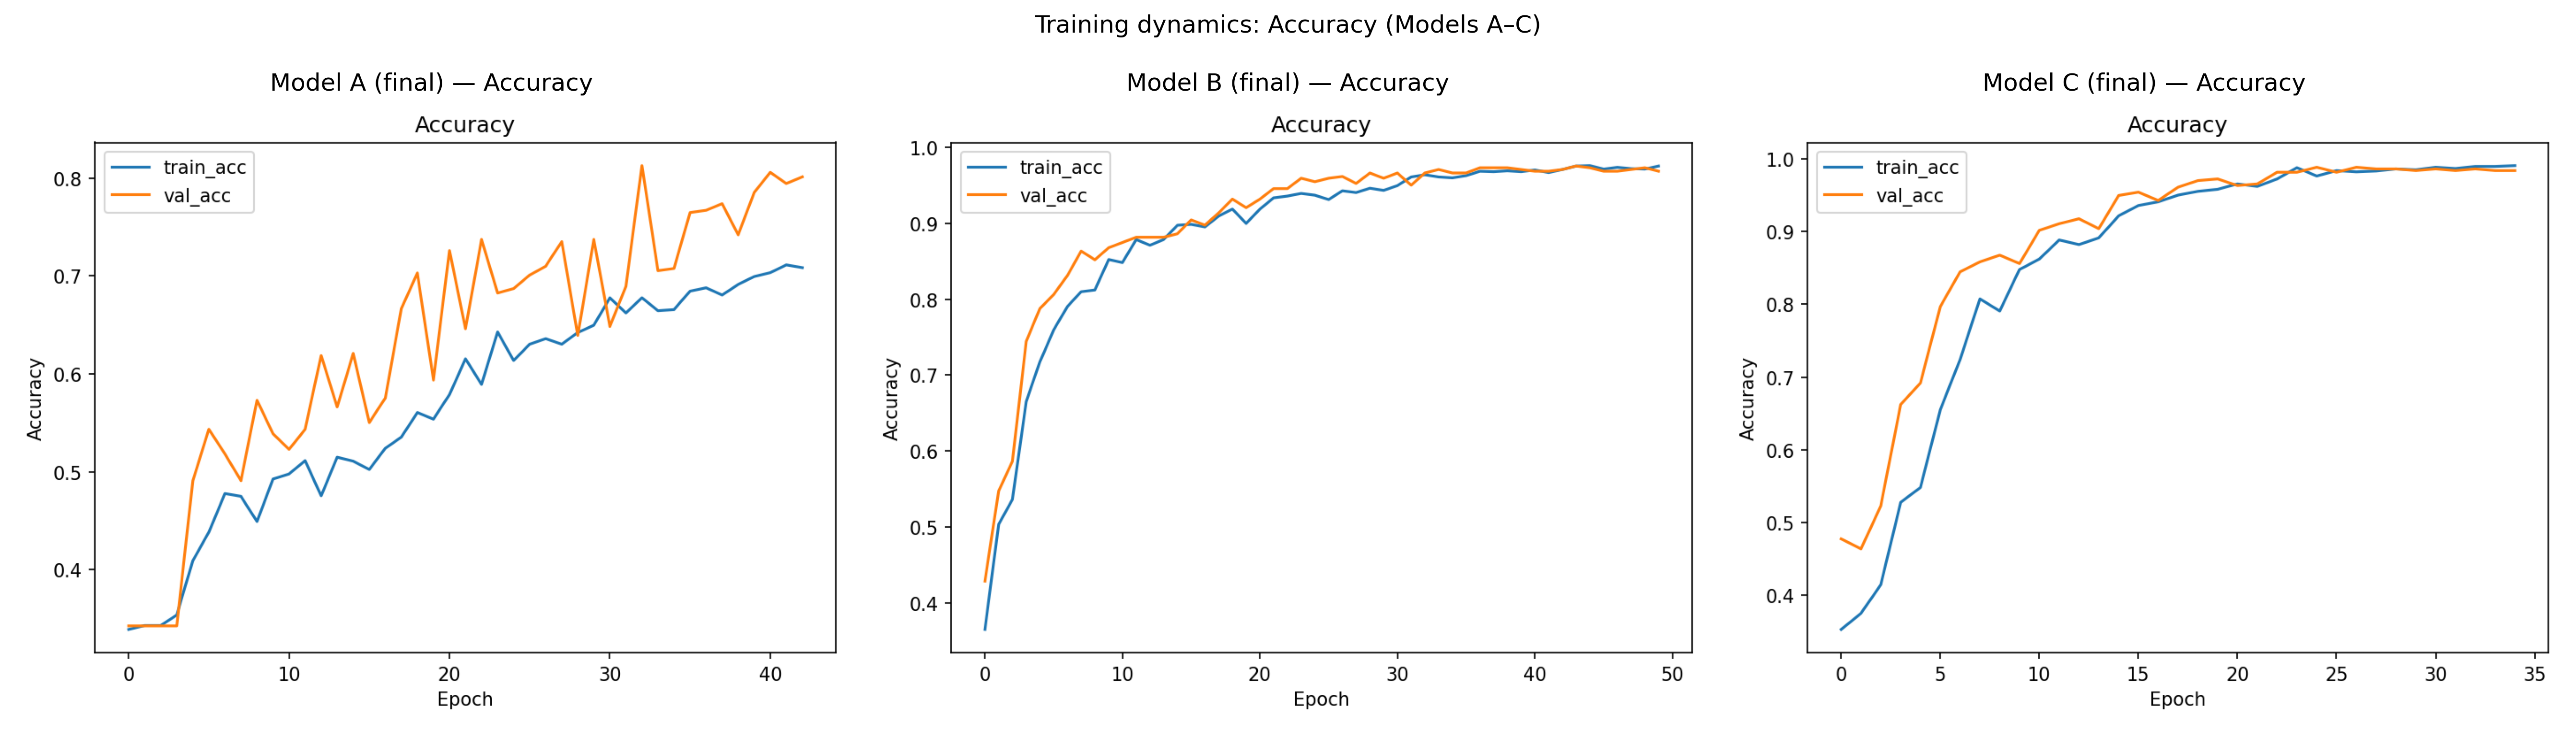
\includegraphics[width=\linewidth]{fig_training_accuracy_all_models.png}

\vspace{0.5cm}

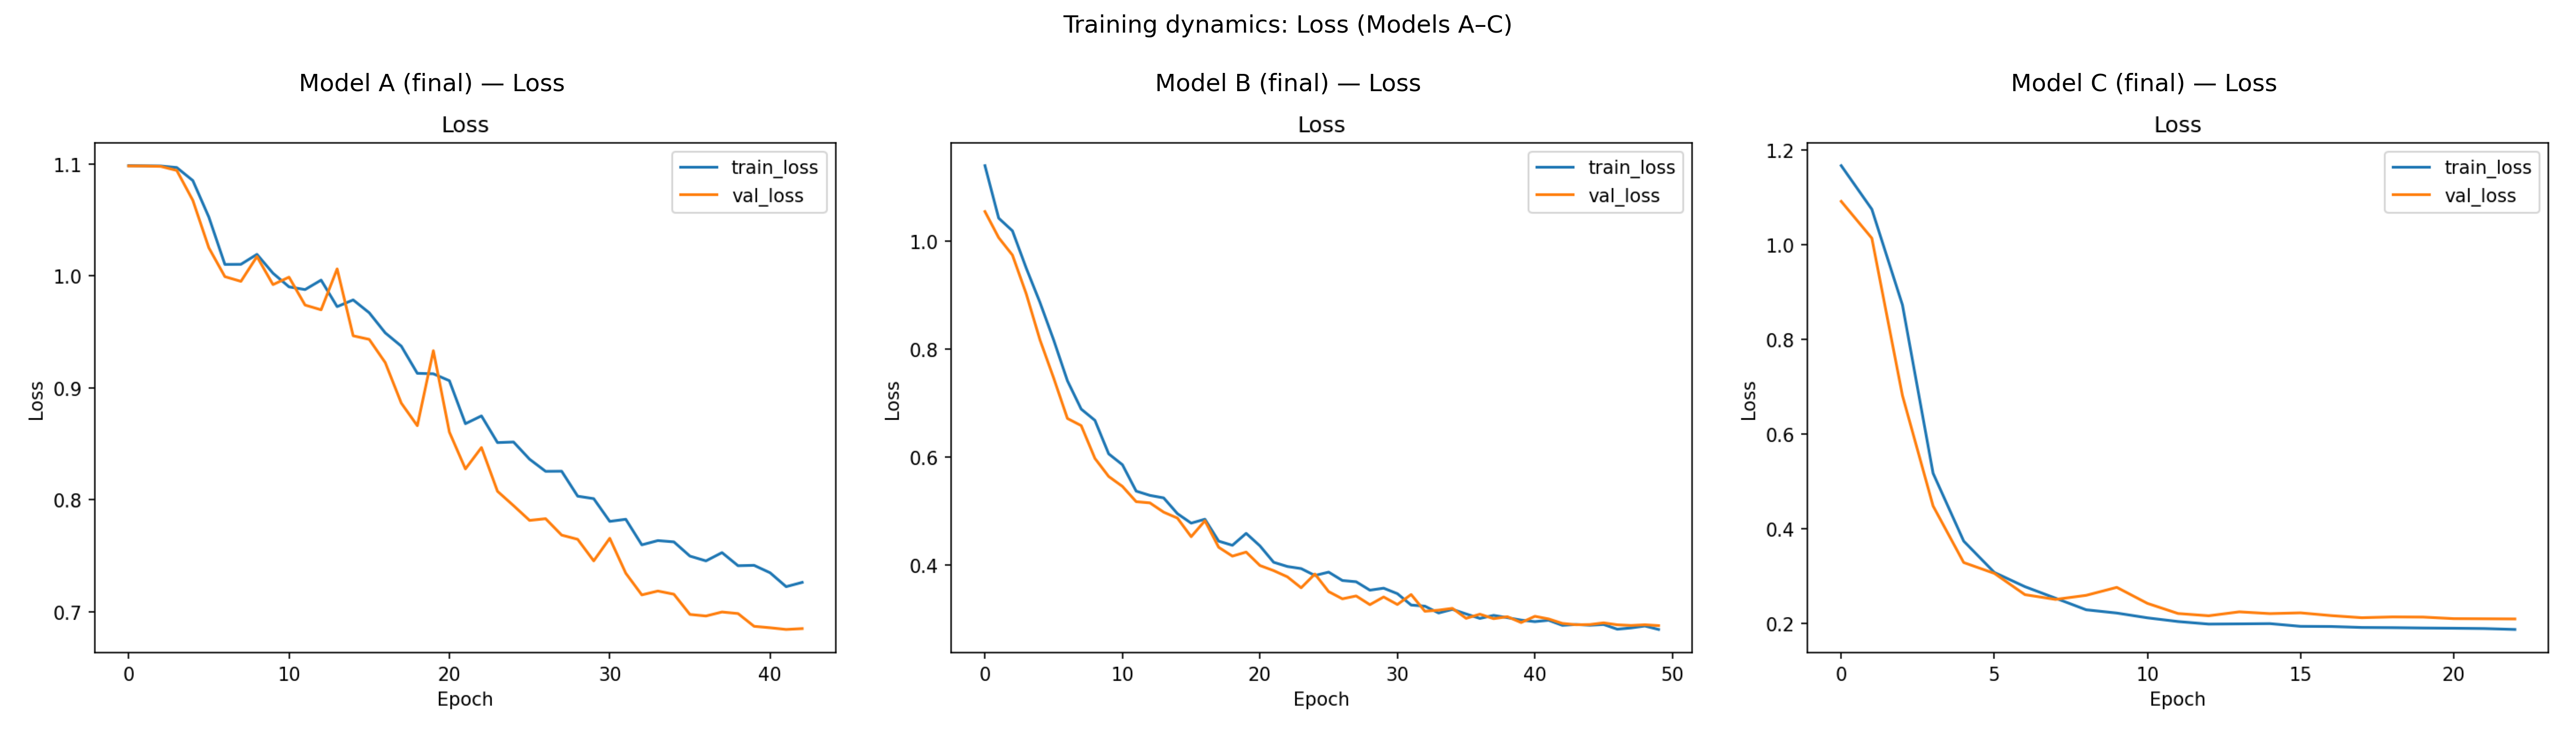
\includegraphics[width=\linewidth]{fig_training_loss_all_models.png}
\caption{Training and validation accuracy (top) and loss (bottom) curves for the three final architectures.}
\label{fig:training_curves}
\end{figure}


For the baseline architecture A, both training and validation loss
decrease smoothly during the initial epochs and gradually approach a plateau, 
while accuracy saturates at relatively low values. The absence of a
widening gap between training and validation curves indicates that the
model does not overfit the data. Instead, the early stagnation of
performance suggests limited representational capacity: the model is
unable to further reduce classification error even on the training set.
In practical terms, this behaviour is characteristic of mild
underfitting, where the architecture captures only coarse visual
patterns and fails to exploit additional training iterations to improve
class discrimination.

Model B exhibits a markedly different learning trajectory. Loss
decreases steadily across epochs for both training and validation sets,
accompanied by a rapid and sustained increase in accuracy. The close
alignment between training and validation curves throughout the
optimization process indicates stable learning and efficient use of
model capacity. From a practical perspective, this pattern suggests that
the architectural enhancements introduced in model B enable the network
to learn more expressive features without sacrificing generalization,
leading to consistent improvements in both error reduction and
predictive accuracy.

Model C shows similarly smooth and stable convergence,but with more rapid 
early error reduction and lower final loss values. Training and
validation curves remain tightly coupled, with only a minimal and
non-systematic generalization gap. This behaviour indicates that the
increased model capacity is effectively controlled through
regularization, allowing the network to fully exploit its expressiveness
without overfitting. In practice, this translates into rapid learning of
highly discriminative representations and stable convergence toward an
optimal solution.

Overall, the progression of training dynamics across models mirrors the
performance trends observed in the classification metrics. Model A is
constrained by insufficient capacity, model B achieves an effective
balance between learning and generalization, and model C combines high
expressiveness with stable optimization. These dynamics confirm that the
observed performance differences are rooted in structural properties of
the architectures rather than in optimization artefacts or training
instability.


\subsection{Analysis of Misclassified Examples}

When informative, a qualitative analysis of misclassified examples was
conducted to identify systematic error patterns and to complement the
quantitative evaluation provided by aggregate performance metrics. In
this context, \emph{misclassified samples} are defined as validation
images for which the predicted class label differs from the ground-truth
label. For each such instance, the predicted class confidence is
computed as the maximum softmax probability associated with the model's
output. This allows misclassifications to be inspected not only in terms
of correctness, but also in terms of model confidence.

To provide a compact overview of class-level error patterns before moving to
instance-level inspection, Figure~\ref{fig:confusion_matrices} reports the
validation confusion matrices for the three final architectures. These
matrices summarize how misclassifications are distributed across classes and
offer a global complement to the analysis presented below.

\begin{figure}[htbp]
\centering

\includegraphics[width=0.32\linewidth]{model_A_final/val_confusion_matrix.png}
\hfill

\includegraphics[width=0.32\linewidth]{model_B_final/val_confusion_matrix.png}
\hfill

\includegraphics[width=0.32\linewidth]{model_C_final/val_confusion_matrix.png}
\caption{Validation confusion matrices for the three final architectures
(models A--C).}
\label{fig:confusion_matrices}
\end{figure}


Misclassified samples are ranked according to their
prediction confidence and a fixed number of the most confident errors is
selected for qualitative inspection. This design choice focuses the analysis on the most
informative failure cases, namely those in which the model assigns high
confidence to an incorrect prediction. Such errors are particularly
relevant, as they reveal systematic confusions in the learned
representation rather than borderline or noisy instances.
Representative misclassified examples for each final architecture are 
shown in the Appendix, Figures~\ref{fig:app_misclf_A}, ~\ref{fig:app_misclf_B} and
~\ref{fig:app_misclf_C}, ordered by decreasing prediction 
confidence.

The qualitative patterns observed differ substantially across
architectures. For Model A, misclassifications are relatively frequent and exhibit a coarse
but systematic structure, consistently with the uneven class-wise recall
reported in Section 3.1. In practical terms, the “missed detections” 
highlighted by the metrics manifest here as a systematic tendency to 
collapse paper and scissors into the rock class: among the most confident 
errors, many true paper and scissors instances are predicted as rock, 
often with high confidence, suggesting reliance on incomplete or misleading 
cues (e.g., coarse hand silhouette and background contrast) rather than 
robust class-defining features. Conversely, true rock appears only rarely 
in this subset, and when it is misclassified it tends to be predicted as 
scissors, indicating an asymmetric error profile where paper and scissors 
are the more challenging classes for this low-capacity representation. 
Overall, these high-confidence mistakes align with the quantitative results 
and training dynamics for Model A, providing further evidence of underfitting.

For model B, misclassified examples become markedly fewer and more
structured. Errors are primarily associated with visually ambiguous
instances, such as partial hand occlusions, non-standard finger
extensions, or poses captured at atypical orientations. Importantly,
these misclassifications tend to occur at lower confidence levels,
suggesting that the model exhibits increased uncertainty when confronted
with borderline cases rather than systematically misinterpreting them.
This pattern reflects a more refined internal representation of gesture
classes and aligns with the balanced precision--recall improvements
observed in the quantitative evaluation.

Misclassifications for model C are rare and highly localized. When
present, they almost exclusively involve intrinsically ambiguous images
in which class boundaries are visually blurred, for example due to
motion blur, extreme perspective, or transitional hand poses between
gestures. Even in these cases, predicted confidence values are generally
lower than those observed for incorrect predictions in simpler
architectures, indicating that the model is aware of its uncertainty.
This behaviour suggests that residual errors are driven by limitations
in the visual signal itself rather than by deficiencies in the learned
representation

In light of the above, the qualitative analysis of misclassified
examples reinforces the conclusions drawn from performance metrics and
training dynamics. As model capacity increases, errors transition from
frequent and unstructured (model A), to rare and ambiguity-driven
(models B and C). This progression indicates that improvements in
classification performance are accompanied by a qualitative shift in the
nature of errors, from representational failures to irreducible visual
ambiguity.

\subsection{Overfitting and Underfitting Assessment}

The presence or absence of overfitting and underfitting was assessed by
jointly analysing quantitative performance metrics, training and
validation learning curves, and the qualitative structure of
classification errors. This combined perspective allows potential
optimization artefacts to be distinguished from genuine limitations in
model capacity.

For the baseline architecture, evidence of underfitting is apparent.
Training accuracy saturates at relatively low levels and does not
continue to improve with additional epochs, while training and
validation loss curves remain closely aligned. This pattern indicates
that the model is unable to sufficiently reduce error even on the
training data, ruling out overfitting and pointing instead to inadequate
representational capacity. The qualitative analysis of misclassified
examples further supports this diagnosis, as errors are frequent and follow 
a strongly biased, asymmetric pattern, suggesting incomplete feature
learning rather than noise sensitivity.

In contrast, no evidence of overfitting is observed for the more
expressive architectures. For both models B and C, training and
validation accuracy curves evolve in parallel, and validation loss does
not exhibit late-stage divergence or instability. The absence of a 
widening generalization gap indicates that performance improvements 
are not driven by memorization of the training data, but rather by the 
learning of representations that generalize reliably within the 
validation distribution. Model C, in particular, combines high
predictive performance with stable optimization behaviour. The minimal
and non-systematic differences between training and validation curves,
together with the rarity and structure of residual errors, suggest that
the model operates in a regime of effective capacity rather than
over-parameterization. Consequently, the selected architecture 
demonstrates robustness under in-distribution conditions. 


\section{Generalization Test}
\subsection{External In-Distribution Evaluation}

In order to disentangle generalization within the same acquisition
domain from robustness to genuine domain shift, the best model (model
C) was additionally evaluated on the \emph{rps-cv-images} dataset. This
dataset is external to the training and validation splits, but shares
similar characteristics in terms of background, lighting conditions, and
gesture presentation.

The model achieves near-perfect performance on this benchmark, with an
overall accuracy exceeding 99\% across 2,188 test images and only a handful of
isolated misclassifications. The confusion matrix is almost perfectly
diagonal, and precision, recall, and F1-scores reach unity for all
classes.
Detailed quantitative results, including the classification report and 
confusion matrix, are provided in Appendix~B.

These results confirm that the selected architecture generalizes
extremely well to unseen data drawn from the same underlying
distribution. 

\subsection{External Out-of-Distribution Evaluation}
\subsubsection{Custom Dataset description}

The custom dataset used for the out-of-distribution evaluation consists
of a small collection of hand gesture images representing the three
target classes (23 images for \emph{rock} and \emph{scissors}, 22 images for \emph{paper}),
acquired outside the original training distribution. The images were
captured using consumer-grade devices under unconstrained conditions and
include hands belonging to multiple individuals rather than a single
subject. This choice introduces natural variability in hand shape, skin
tone, finger proportions, and gesture execution style, thereby
increasing the heterogeneity of the dataset.

In addition to subject variability, the images exhibit substantial
diversity in background, lighting conditions, and viewpoint. Backgrounds
range from uniform surfaces to textured environments such as wooden
floors, tiled areas, and indoor furnishings, while lighting conditions
vary from diffuse natural light to indoor artificial illumination. The
hand poses are not strictly canonical: gestures may be partially
rotated, cropped, or captured at non-standard distances and angles.
Accessories such as watches or wristbands are also present in some
images, further increasing visual complexity.

Although the dataset is approximately class-balanced, it is
intentionally small and uncurated, reflecting realistic acquisition
conditions rather than controlled laboratory settings. As such, it is
not intended to provide statistically robust performance estimates, but
rather to serve as a qualitative stress test for model robustness and
generalization under domain shift. The dataset allows for a focused
analysis of how well models trained on clean, curated data transfer to
real-world scenarios characterized by higher intra-class variability and
reduced visual consistency.

\subsubsection{Out-of-Distribution Evaluation on Custom Data}

The evaluation on the custom hand-gesture dataset highlights a clear and
systematic difference in robustness across the three architectures under
out-of-distribution conditions. Despite the dataset being nearly
class-balanced, models A and B exhibit a pronounced bias towards the
\emph{scissors} class, as evidenced by highly skewed predicted class
distributions and extreme mean predicted priors. In particular, model B
collapses almost entirely onto \emph{scissors} (predicted prior $\approx$
{[}0.003, 0.001, 0.996{]}), while model A shows a slightly milder but
still substantial preference for the same class.

This behaviour is reflected in their confusion matrices and per-class
metrics, where \emph{scissors} achieves comparatively higher F1-scores
than \emph{rock} and especially \emph{paper} for models A and B, with
\emph{paper} being strongly penalized (Table~\ref{tab:custom_eval_f1_per_class}).
This pattern indicates that, under domain shift, the simpler architectures
systematically favour the most visually distinctive class, improving
performance on \emph{scissors} at the expense of degraded discrimination
between \emph{rock} and \emph{paper}. The corresponding misclassified-image
grids further reveal that visually ambiguous \emph{rock} and \emph{paper}
gestures are consistently mapped to \emph{scissors} with high confidence,
supporting the interpretation of a bias-driven error structure rather than
class-specific noise.

\begin{table}[h]
\centering
\caption{Per-class F1-score on the custom hand-gesture dataset.}
\label{tab:custom_eval_f1_per_class}
\begin{tabular}{lccc}
\hline
Model & F1 (rock) & F1 (paper) & F1 (scissors) \\
\hline
A & 0.318 & 0.077 & 0.455 \\
B & 0.188 & 0.167 & 0.382 \\
C & 0.458 & 0.509 & 0.364 \\
\hline
\end{tabular}
\end{table}

Model C, while not immune to domain shift, substantially mitigates this
failure mode. In terms of top-1 decisions, it avoids degenerating into a
single-class predictor and yields higher overall accuracy and macro F1-score,
with a confusion matrix that preserves meaningful structure. 
Although the average predicted probability assigned to 
\emph{scissors} is close to zero before recalibration (Appendix~C, 
Table~\ref{tab:app_custom_pred_priors}), the confusion matrix 
shows that the model still assigns \emph{scissors} as the top-1 label for 
some samples. This indicates a calibration/score-shift effect, rather than a complete 
collapse in which the argmax always selects a single class.

These trends are summarized quantitatively by the macro-averaged evaluation 
metrics reported in Table~\ref{tab:custom_eval_metrics} and are visually 
corroborated by the confusion matrices in Appendix~C 
(Figure~\ref{fig:app_custom_confusion_combined}), which clearly illustrate the 
systematic class collapse observed for models A and B and its mitigation in model C.

\begin{table}[h]
\centering
\caption{Custom hand-gesture dataset evaluation by model. Metrics are macro-averaged over classes.}
\label{tab:custom_eval_metrics}
\begin{tabular}{lcccc}
\hline
Model & Accuracy & Macro Precision & Macro Recall & Macro F1 \\
\hline
A & 0.338 & 0.311 & 0.334 & 0.283 \\
B & 0.279 & 0.279 & 0.277 & 0.246 \\
C & 0.456 & 0.488 & 0.458 & 0.444 \\
\hline
\end{tabular}
\end{table}


Overall, these results suggest that increased representational capacity
and architectural regularization improve robustness to real-world
variability, while also highlighting the intrinsic difficulty of
reliably distinguishing hand gestures under uncontrolled acquisition
conditions. 

\section{Conclusion and Future Work}

This project investigated how increasing architectural complexity in
convolutional neural networks affects both predictive performance and
robustness to distributional shift in image classification tasks, using
rock--paper--scissors hand gesture recognition as a controlled case study.
Through a systematic comparison of three CNN architectures trained under identical
optimization settings, the analysis demonstrated a clear relationship
between model capacity and predictive performance. While the baseline
architecture exhibited signs of underfitting and limited discriminative
power, progressively deeper and better-regularized models achieved very
strong in-distribution performance, confirming the benefits of increased
representational expressiveness for this task.

Beyond in-distribution evaluation, the study placed particular emphasis
on model robustness under domain shift by introducing an external test
set composed of unconstrained, real-world hand gesture images. This
generalization test revealed that simpler architectures tend to collapse
toward visually dominant classes when confronted with unfamiliar
acquisition conditions, leading to highly skewed predictions and poor
class balance. In contrast, the most expressive model retained a more
structured decision behaviour and substantially mitigated this failure
mode, although some degradation in confidence calibration remained.
These findings highlight that strong in-distribution validation performance alone is not
sufficient to guarantee robustness in real-world scenarios and
underscore the importance of explicitly evaluating models under
out-of-distribution conditions.

Despite these encouraging results, several limitations must be
acknowledged. The custom dataset used for the generalization test is
intentionally small and qualitative in nature, preventing statistically
robust performance estimates and limiting the strength of conclusions that can be drawn about 
generalization under domain shift. Moreover, all models were trained
exclusively on a curated dataset, without the use of advanced data
augmentation strategies or domain adaptation techniques that could
further enhance robustness. 

Future work could therefore explore the impact of more aggressive augmentation
pipelines and the inclusion of real-world images during training to improve
generalization under domain shift. Additionally, future experiments could
evaluate the use of models pretrained on large image datasets to further
enhance robustness in out-of-distribution settings. Investigating probabilistic
calibration methods and confidence-aware decision mechanisms could also help
address residual uncertainty when models are deployed in unconstrained
environments.

Finally, in terms of potential applications, the final model could be deployed
as a lightweight web application enabling interactive rock--paper--scissors play
and real-time qualitative evaluation.

\newpage
\appendix
\section*{Appendix}
\addcontentsline{toc}{section}{Appendix}

\section{Additional Qualitative Diagnostics}
\subsection{Misclassified examples}

Images are ranked by decreasing prediction confidence. Each panel reports the true label (T), the predicted label (P), and the associated softmax confidence score.

\newcommand{\misclfimgAB}[1]{%
  \includegraphics[
    width=0.92\linewidth,
    height=0.50\textheight,
    keepaspectratio
  ]{#1}
}

\newcommand{\misclfimgC}[1]{%
  \includegraphics[
    width=0.85\linewidth,
    height=0.35\textheight,
    keepaspectratio
  ]{#1}
}

\begin{figure}[!htbp]
    \centering
    \misclfimgAB{model_A_final/val_misclassified.png}
    \caption{Most confident misclassified validation samples for \textbf{Model A}.}
    \label{fig:app_misclf_A}
\end{figure}

\begin{figure}[!htbp]
    \centering
    \misclfimgAB{model_B_final/val_misclassified.png}
    \caption{Most confident misclassified validation samples for \textbf{Model B}.}
    \label{fig:app_misclf_B}
\end{figure}

\begin{figure}[!htbp]
    \centering
    \misclfimgC{model_C_final/val_misclassified.png}
    \caption{Most confident misclassified validation samples for \textbf{Model C}.}
    \label{fig:app_misclf_C}
\end{figure}

\FloatBarrier

\section{External In-Distribution Evaluation Details}

\subsection{Classification report}

\begin{table}[!htbp]
\centering
\caption{Classification report for model C on the external in-distribution test set \emph{rps-cv-images} (rounded values).}
\label{tab:app_test_classification_report}
\begin{tabular}{lcccc}
\hline
\textbf{Class} & \textbf{Precision} & \textbf{Recall} & \textbf{F1-score} & \textbf{Support} \\
\hline
Rock      & 1.00 & 1.00 & 1.00 & 726 \\
Paper     & 1.00 & 1.00 & 1.00 & 712 \\
Scissors  & 1.00 & 1.00 & 1.00 & 750 \\
\hline
Accuracy      &      &      & 1.00 & 2188 \\
Macro avg     & 1.00 & 1.00 & 1.00 & 2188 \\
Weighted avg  & 1.00 & 1.00 & 1.00 & 2188 \\
\hline
\end{tabular}
\end{table}

\FloatBarrier 

\subsection{Confusion matrix}

\begin{figure}[!htbp]
    \centering
    
\includegraphics[width=0.6\linewidth]{model_C_final/test_confusion_matrix.png}
    \caption{Confusion matrix for model C on the external in-distribution test set (\emph{rps-cv-images}).}
    \label{fig:app_test_confusion}
\end{figure}

\section{External Out-Of-Distribution Evaluation Details}

\subsection{Confusion matrices}

\begin{figure}[!htbp]
\centering
\includegraphics[width=0.9\linewidth]{custom_eval_myhands/confusion_matrices_custom_combined.png}
\caption{Confusion matrices for the three architectures evaluated on the custom out-of-distribution dataset.}
\label{fig:app_custom_confusion_combined}
\end{figure}

\FloatBarrier

\subsection{Predicted class priors}

\begin{table}[!htbp]
\centering
\caption{Mean predicted class priors (pre-recalibration) for the three architectures on the custom out-of-distribution dataset.}
\label{tab:app_custom_pred_priors}
\begin{tabular}{lccc}
\hline
\textbf{Model} & \textbf{Rock} & \textbf{Paper} & \textbf{Scissors} \\
\hline
Model A & 0.066 & 0.074 & 0.860 \\
Model B & 0.003 & 0.001 & 0.996 \\
Model C & 0.332 & 0.668 & 0.000 \\
\hline
Target prior & 0.333 & 0.333 & 0.333 \\
\hline
\end{tabular}
\end{table}



\end{document}
